\documentclass{article}

% tight measures:
% \usepackage[margin=0mm, paperwidth=77.9mm, paperheight=72.1mm]{geometry}
% loose measures:
\usepackage[margin=2mm, paperwidth=81.9mm, paperheight=76.1mm]{geometry}

\usepackage{amsmath}
\usepackage{tikz}
\usetikzlibrary{bayesnet}
\usepackage{bm}
\providecommand{\mathbold}[1]{\bm{#1}}
\newcommand{\vct}[1]{\mathbold{#1}}

\begin{document}
\thispagestyle{empty}

\begin{center}
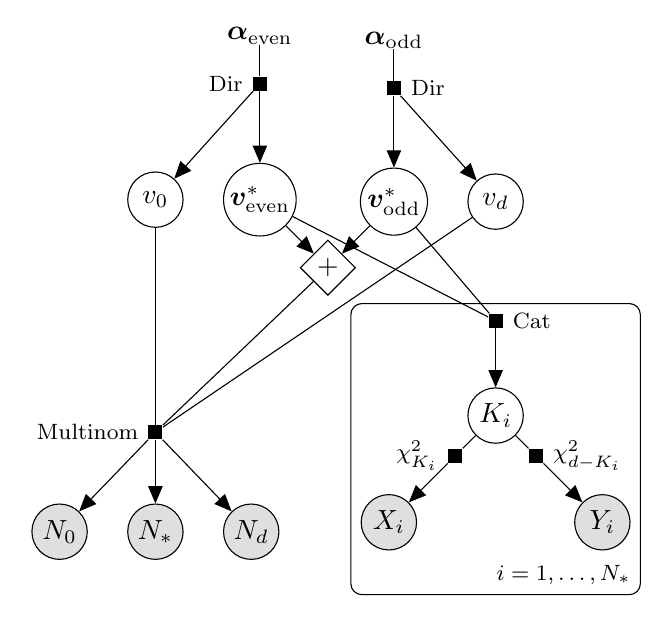
\begin{tikzpicture}
   \node[det] (sum) {$+$} ;
   \node[latent, above left=.5 of sum] (veven) {$\vct{v}_{\text{even}}^*$} ;
   \node[latent, left=.5 of veven] (v0) {$v_0$} ;
   \node[latent, above right=.5 of sum] (vodd) {$\vct{v}_{\text{odd}}^*$} ;
   \node[latent, right=.5 of vodd] (vd) {$v_d$} ;
   
   \node[const, above=1.5 of veven] (alpha) {$\vct{\alpha}_{\text{even}}$} ;
   \node[const, above=1.5 of vodd] (beta) {$\vct{\alpha}_{\text{odd}}$} ;
   \factor[below=of alpha] {alp-f} {left:Dir} {alpha} {v0,veven} ;
   \factor[below=of beta] {bet-f} {right:Dir} {beta} {vodd,vd} ;

   \edge[->] {veven,vodd} {sum} ;
   
   \node[obs, below=3.5 of v0] (bulk) {$N_*$} ;
   \node[obs, left=.5 of bulk] (p0) {$N_0$} ;
   \node[obs, right=.5 of bulk] (pd) {$N_d$} ;
   \factor[below=2.5 of v0] {extr-f} {left:Multinom} {v0,sum,vd} {bulk,p0,pd} ;
   
   \node[latent, below=2 of vd] (K) {$K_i$} ;
   \node[obs, below left=1.2 of K] (X) {$X_i$} ;
   \node[obs, below right=1.2 of K] (Y) {$Y_i$} ;
   \factor[above right=.7 of X] {X-f} {left:$\chi_{K_i}^2$} {K} {X} ;
   \factor[above left=.7 of Y] {Y-f} {right:$\chi_{d-K_i}^2$} {K} {Y} ;
   \factor[above=.75 of K] {K-f} {right:Cat} {veven,vodd} {K} ;

   \plate {KXY} {(K)(K-f)(X)(Y)} {$i=1,\ldots,N_*$} ;
\end{tikzpicture}
\end{center}

\end{document}











